\subsection{L1L1}

The L1L1 dataset in the 1.5~mm data includes vertices reconstructed from pairs of tracks that have hits in Layer 1 of the SVT. Due to the SVT opening being larger, the acceptance favors larger heavy photon masses. The SVT has also lower rates in Layer 1 when compared to the 0.5~mm dataset.


\subsubsection{Cuts}

The cuts applied to the L1L1 dataset are shown in Table~\ref{l1l1_cuts_1p5}.

\begin{table}[H]
\caption{Cuts applied to the L1L1 datasets with the SVT at 1.5mm.}
\label{l1l1_cuts_1p5}
\centering
\begin{tabular}{llllll}
\toprule
%\multicolumn{2}{c}{Name} \\
%\cmidrule(r){1-2}
Cut type & Cut & Cut Value &  $\%$killed &  $\%$killed core & $\%$killed tails\\
\midrule
track & Fit quality & track $\chi^{2}<30$ & 37 & 22 & 87 \\
track & Max track momentum &  $P_{trk}<75\%E_{beam}$ & 6 & 6 & 19 \\
track & Isolation &   & 2 & 1 & 15 \\
vertex & beamspot constraint & bsc$\chi^{2}<10$  & 23 & 21 & 81 \\
vertex & beamspot - unconstrained & bsc$\chi^{2}$-unc$\chi^2<5$  & 12 & 12 & 27 \\
vertex & maximum $P_{sum}$ &  $<115\%E_{beam}$ & 0 & 0 & 2 \\
ecal & Ecal SVT matching & $\chi^2<10$  & 3 & 3 & 58 \\
ecal & track Ecal timing & $<4$ns  & 5 & 5 & 7 \\
ecal & 2 cluster time diff & $<2$ns  & 4 & 4 & 13 \\
physics & momentum asymmetry & $<0.4$  & 12 & 12 & 48 \\
physics & e+ track d0 & $<1.5$mm  & 0 & 0 & 4 \\
event & max shared hits amongst tracks & $<5$ shared hits  & 12 & 12 & 20 \\
\bottomrule
\end{tabular}
\end{table}

The cuts are the same as those applied to the 0.5~mm dataset with similar effect.

\subsubsection{Vertex reconstruction efficiency, $\epsilon_{vtx}$}

The efficiency of the 1.5~mm data was obtained using the same methodology as the 0.5~mm data. Using heavy photon simulation at fixed masses, one can compared the reconstructed heavy photons as a function of vertex position for all datatsets. The reconstuced vertex efficiency at the at the target for the L1L1 dataset is scaled to 1, and the L1L2 and L2L2 datasets are scaled, accordingly. The resulting efficiency effect can be seen in Figure~\ref{fig:eff1p5mm}.

\begin{figure}[H]
  \centering
     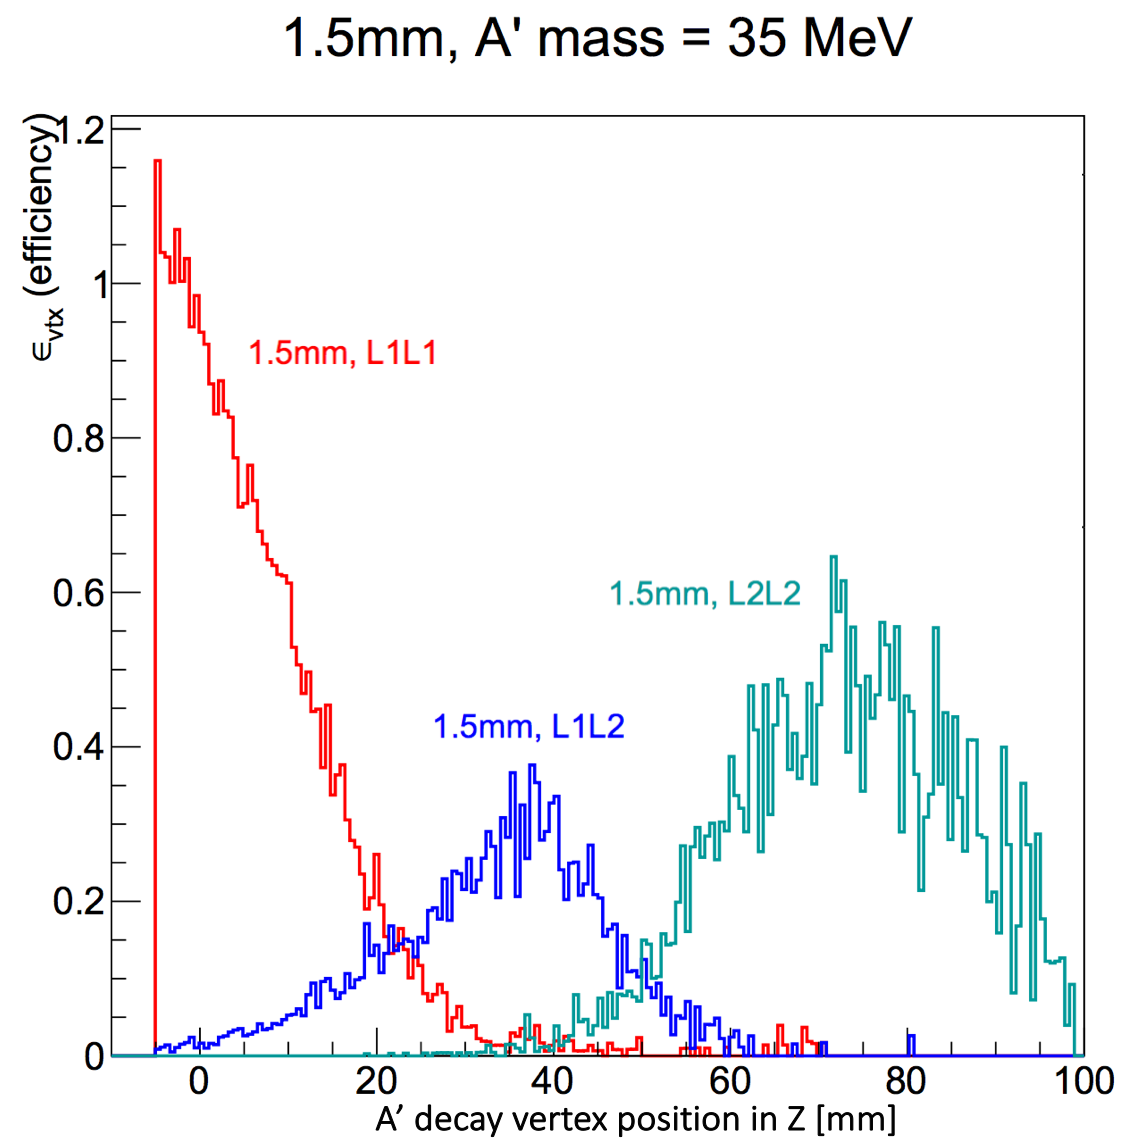
\includegraphics[width=0.8\textwidth]{plots/Effplots_1p5.png}
  \caption{35~MeV reconstruction efficiency versus the vertex position. }
  \label{fig:eff1p5mm}
\end{figure} 

The L1L1 efficiency for each mass was fit using Equation~\eqref{eq:epsVtxL1_1p5}. 

\begin{equation}
\label{eq:epsVtxL1_1p5}
\epsilon_{vtx} = exp(p_0z^3+p_1z^2+p_2z+p_3) 
\end{equation}

 The parameters of Equation~\eqref{eq:epsVtxL1_1p5} are then studied as a function of mass as shown in Equation~\eqref{eq:epsVtxL1_1p5}.

\begin{eqnarray*}
\label{eq:parsEpsVtxL1_1p5}
p_0 & = & 1.034E-5-1.2E-7m \\
p_1 & = & -0.00324+0.00016m \\
p_2 & = & 0.0412-0.0037m+4.11E-5m^2 \\
p_3 & = & -0.1348+0.000784m \\
\end{eqnarray*}

The vertex reconstruction efficiency can then be applied to the integral in Equation~\eqref{eq:signal}. The value of the integral yields the fraction of measured heavy photon signal events. For the L1L1 dataset, the zMax value is 100~mm, and the integral values for various zCuts is shown in Figure~\ref{fig:Inteff_L1L1_1p5}.

\begin{figure}[H]
  \centering
     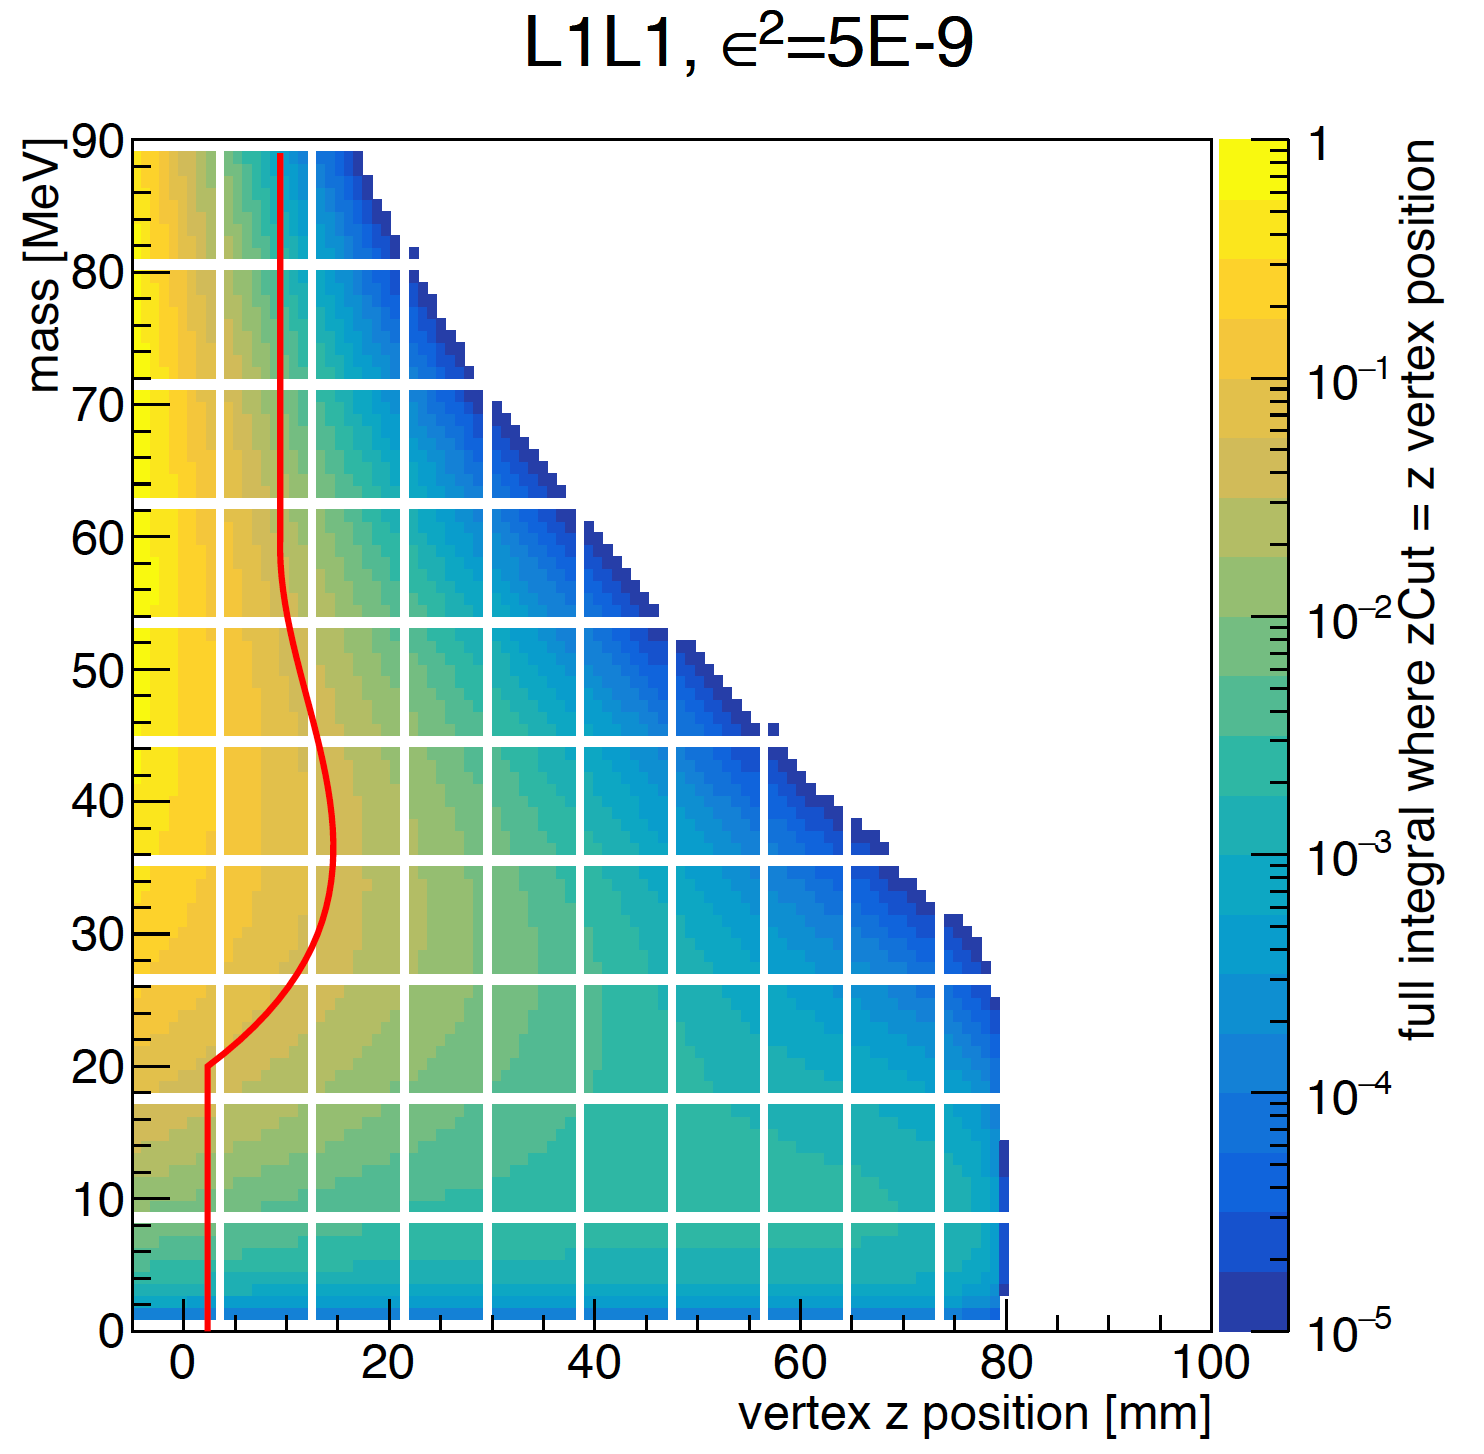
\includegraphics[width=0.8\textwidth]{plots/L1L1_eff1p5_zm.png}
  \caption{The colored value is the value of the full integral from Equation~\ref{eq:signal} for the L1L1 1.5~mm dataset using the zCut value on the x-axis. The red line indicates the zCut value derived in data for 0.5 background events. The zCut shown is for the 10$\%$ unblinded data.}
  \label{fig:Inteff_L1L1_1p5}
\end{figure} 

 We can see the full integral value for various couplings across a range of masses in the dataset in Figure~\ref{fig:IntCoup_L1l1}.

\begin{figure}[H]
  \centering
     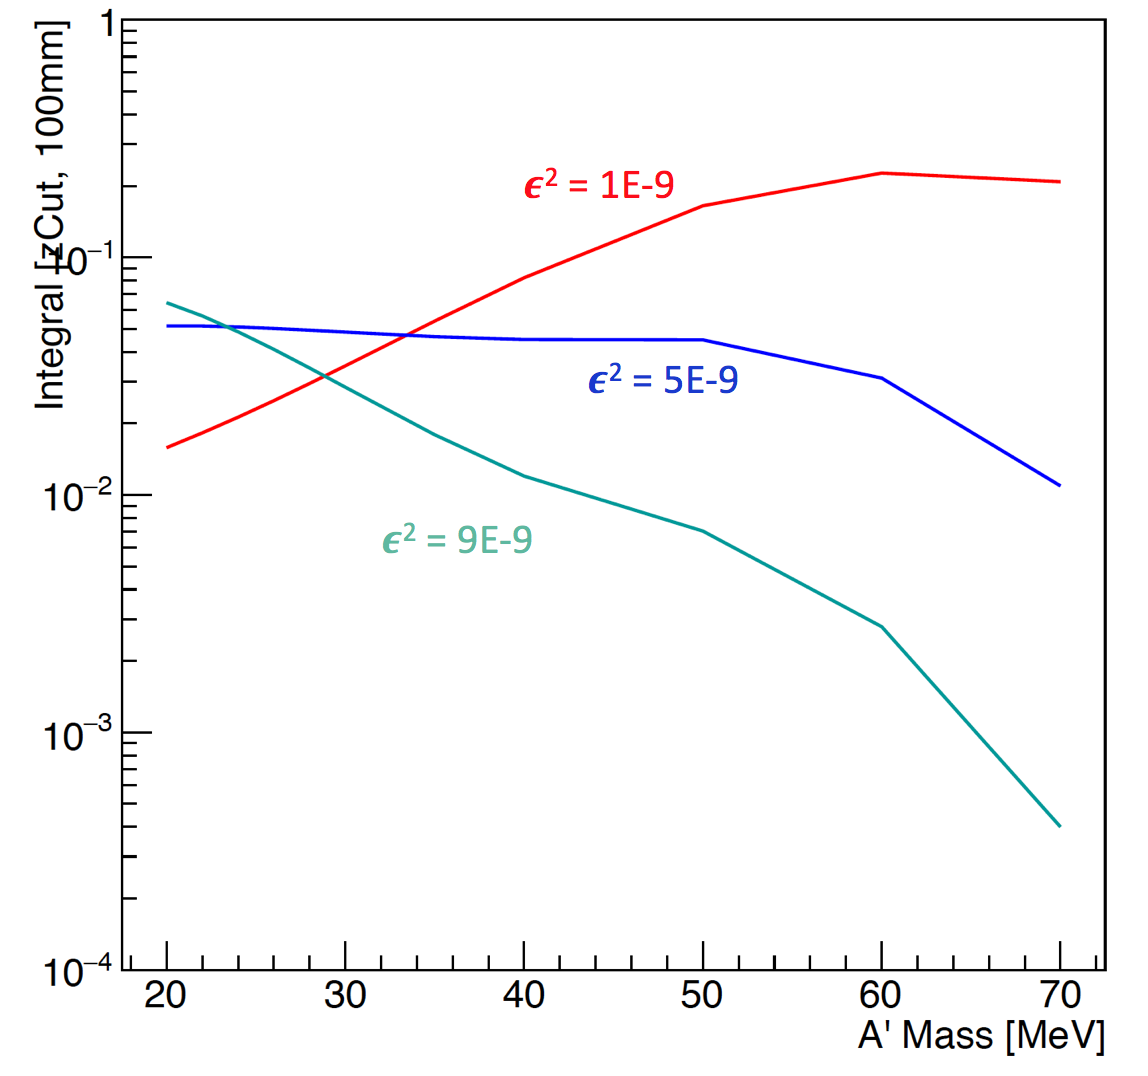
\includegraphics[width=0.8\textwidth]{plots/integratedEff_1p5.png}
  \caption{For the measured zCut value in the 10$\%$ of the data, the corresponding integral value for various couplings across a range of masses is shown.}
  \label{fig:IntCoup_L1l1}
\end{figure} 

The mass resolution has been shown previously to be nearly the same between 0.5~mm and 1.5~mm datasets. 

\subsubsection{Accidentals}

When counting the reconstructed vertices having cluster time differences between 3 and 9~ns apart, no high z events were produced. It's possible that the statistics are too low to say with any certainty that we will not see any when unblinding, but this does seem to indicate that we should see no accidental events in the 10$\%$ unblinded sample currently studied.

\subsubsection{Projected reach}

The resultant vertex distribution as a function of mass is shown in Figure~\ref{fig:zVm_L1L1_1p5}. 

\begin{figure}[H]
  \centering
     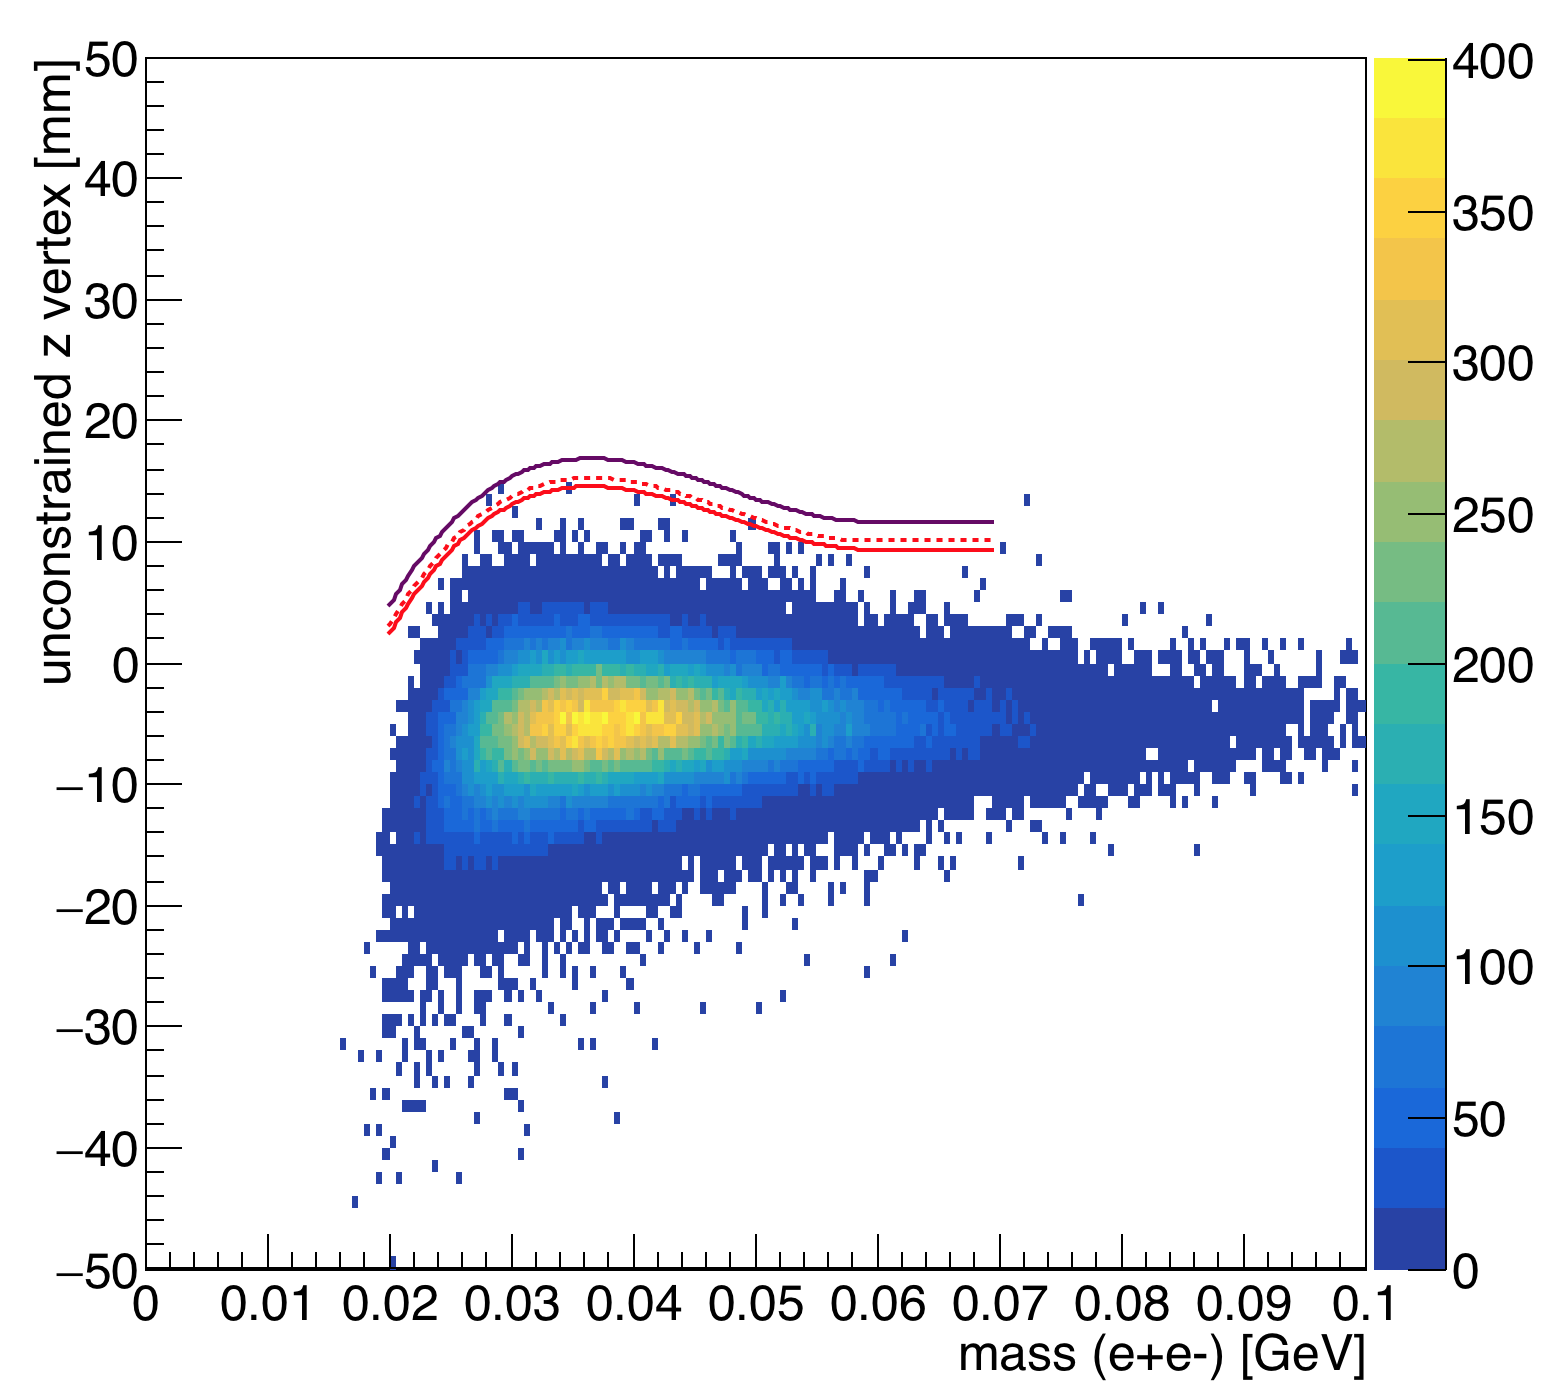
\includegraphics[width=0.8\textwidth]{plots/zVm_L1L1_1p5.png}
  \caption{Reconstructed z vertex as a function of mass for the L1L1 dataset with the first layer of the SVT at 1.5~mm from the beam. The solid red line indicates the zCut found for 10$\%$ of the data (unblinded), and the dashed red line indicates the limit at which events have a quantile greater than 0.5 with respect to the predicted background model. The purple line shows where the projected zCut will be for the full dataset after unblinding.}
  \label{fig:zVm_L1L1_1p5}
\end{figure} 

The reach projections for the 1.5~mm dataset include the statistics of the 0.5~mm dataset in the value of $N_bin$ as described by Equation~\ref{eq:signal}. The reach projection for the L1L1 1.5~mm dataset is shown in Figure~\ref{fig:reach1p5}.

\begin{figure}[H]
  \centering
     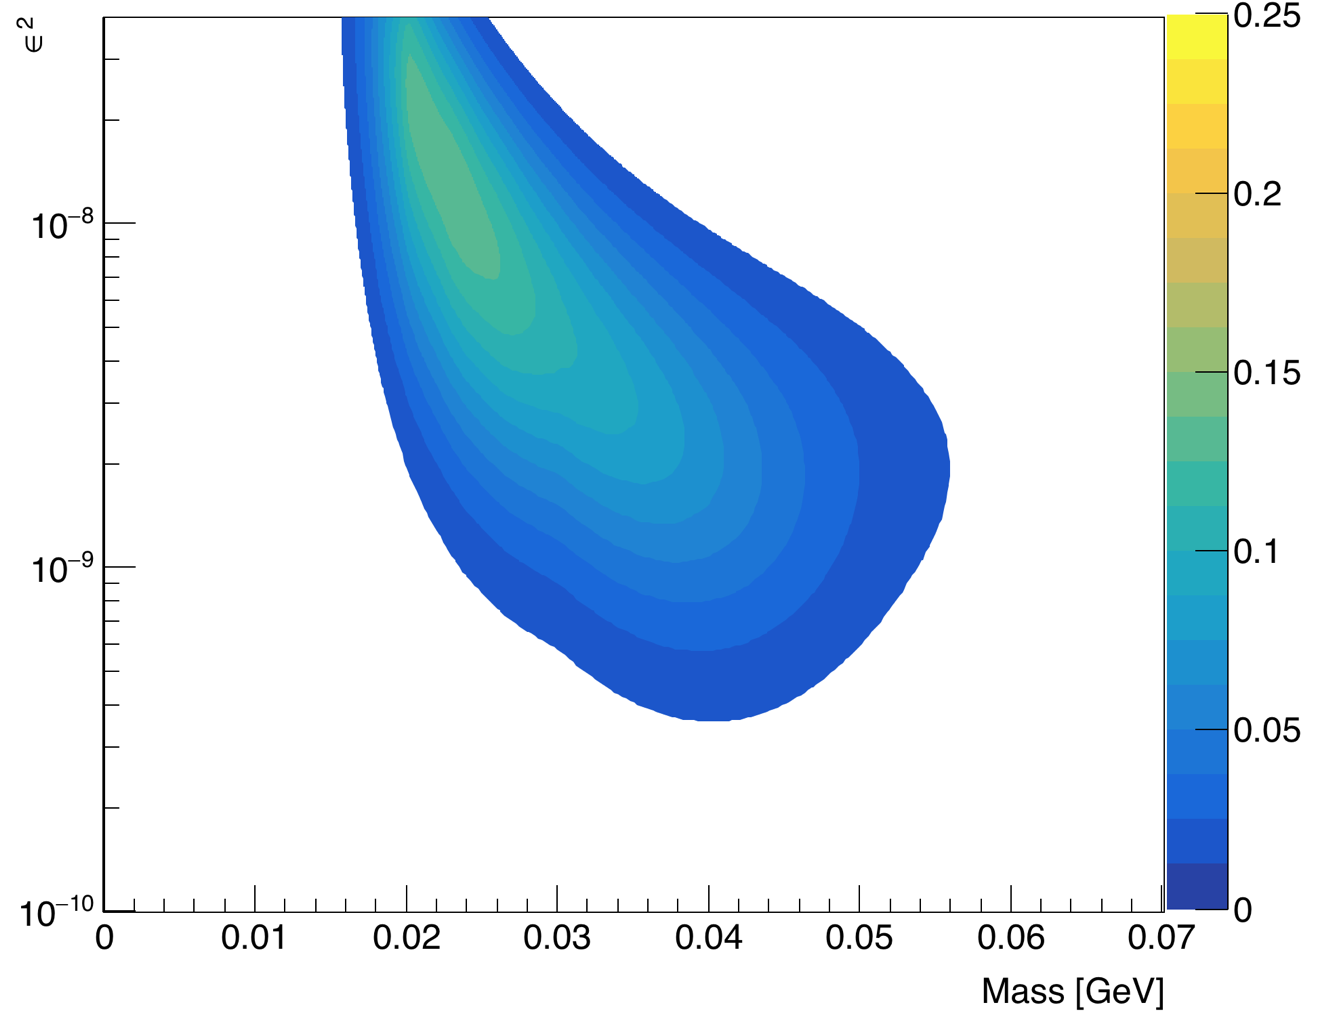
\includegraphics[width=0.8\textwidth]{plots/reachL1L1_1p5.png}
  \caption{The expected signal yield for the full 100$\%$ dataset with L1L1 1.5~mm data.}
  \label{fig:reach1p5}
\end{figure} 

Here we see that the reach is most sensitive to largely coupled, smaller mass decays due to the larger opening of the SVT. 
